\documentclass[a4paper, 11pt, twoside, fleqn]{memoir}

\usepackage{AOCDTF}

%%--------------------------------------
%entrées du glossaire
%--------------------------------------

%création de macro-commande pour automatiser la rédaction de nouvelles entrées référencés dans le glossaire

\newglossaryentry{ex}{name={exemple}, description={définition de l'exemple d'entrée classique dans le glossaire}}
%%--------------------------------------
%entrées des acronymes
%--------------------------------------

\newacronym{aocdtf}{AOCDTF}{Association Ouvrière des Compagnons du Devoir et du Tour de France}

\newacronym{ide}{IDE}{Environnement de Développement (Integrated Development Environment)}

\newacronym{isq}{ISQ}{International System of Quantities}

\newacronym{usi}{USI}{Unité du Système International}

\newacronym{si}{SI}{Système International}


\typemedia{paper} %choix screen ou paper pour les vidéos et schémas animés

\decoupagechapitre{1} %juste pour éviter les erreurs lors de la compilation des sous-programmations (passera en commentaire)
\marqueurchapitre

%lien d'édition des figures Tikz sur le site mathcha.io (rajouter le lien d'une modification effectuée sur la figure tikz avec le nom du modificateur car il n'y a qu'un lien par compte)

%lien mathcha Nom Prénom : 

%--------------------------------------
%corps du document
%--------------------------------------

\begin{document} %corps du document
	\openleft %début de chapitre à gauche

\begin{landscape}
\begin{longtableau}{\linewidth}{l O c c c X X c c }{10}{Portes logiques}
{& \multicolumn{2}{c}{\thead{\'Equation logique}}	& \multicolumn{3}{c}{\thead{Table de vérité}}	&	\thead{Identité remarquable}	& \thead{Propriété}	& \thead{Symbole} 	& 	\thead{Schéma}\\}
\multicolumn{10}{l}{Fonction OUI} \\
\middashrule
 & S	&	a	&	& a	&	S	&	& &	\multirow[c]{3}{*}{\adjustbox{valign=t}{


\tikzset{every picture/.style={line width=0.75pt}} %set default line width to 0.75pt        

\begin{tikzpicture}[x=0.75pt,y=0.75pt,yscale=-1,xscale=1]
%uncomment if require: \path (0,300); %set diagram left start at 0, and has height of 300

%Shape: Rectangle [id:dp961707875303309] 
\draw   (80,30) -- (125,30) -- (125,90) -- (80,90) -- cycle ;
%Straight Lines [id:da9680164160115489] 
\draw    (125,60) -- (155,60) ;
%Straight Lines [id:da6569354332271061] 
\draw    (50,60) -- (80,60) ;


% Text Node
\draw (78,57) node [anchor=south east] [inner sep=0.75pt]   [align=left] {a};
% Text Node
\draw (127,57) node [anchor=south west] [inner sep=0.75pt]   [align=left] {S};


\end{tikzpicture}}}


&

\multirow[c]{3}{*}{\adjustbox{valign=t}{
\tikzset{every picture/.style={line width=0.75pt}} %set default line width to 0.75pt        

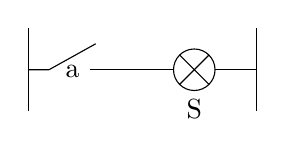
\begin{tikzpicture}[x=0.75pt,y=0.75pt,yscale=-1,xscale=1]
%uncomment if require: \path (0,300); %set diagram left start at 0, and has height of 300

%Straight Lines [id:da2327596890580329] 
\draw    (122.5,67.5) -- (100,80) -- (90,80) ;
%Straight Lines [id:da7293492467717119] 
\draw    (120,80) -- (130,80) ;

%Straight Lines [id:da745902934682585] 
\draw    (90,60) -- (90,100) ;
%Straight Lines [id:da6994104941060462] 
\draw    (130,80) -- (160,80) ;
%Flowchart: Summing Junction [id:dp7647527049013112] 
\draw   (160,80) .. controls (160,74.48) and (164.48,70) .. (170,70) .. controls (175.52,70) and (180,74.48) .. (180,80) .. controls (180,85.52) and (175.52,90) .. (170,90) .. controls (164.48,90) and (160,85.52) .. (160,80) -- cycle ; \draw   (162.93,72.93) -- (177.07,87.07) ; \draw   (177.07,72.93) -- (162.93,87.07) ;
%Straight Lines [id:da5758872070263168] 
\draw    (180,80) -- (200,80) ;
%Straight Lines [id:da13301424795036298] 
\draw    (200,60) -- (200,100) ;

% Text Node
\draw (170,93) node [anchor=north] [inner sep=0.75pt]   [align=left] {S};
% Text Node
\draw (111.25,76.75) node [anchor=north] [inner sep=0.75pt]   [align=left] {a};


\end{tikzpicture}}}
\\
\cmidrule(lr){4-6}
& \multicolumn{2}{c}{} & & 0 & 0 & & & & \\
& \multicolumn{2}{c}{} & & 1 & 1 & & & & \\








\multicolumn{10}{l}{Fonction NON} \\
\middashrule
 & S	&\bar{a}	&	& a	&	S	&	& &	\multirow[c]{3}{*}{\adjustbox{valign=t}{




\tikzset{every picture/.style={line width=0.75pt}} %set default line width to 0.75pt        

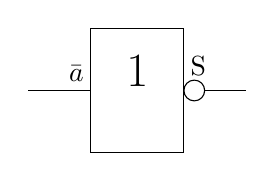
\begin{tikzpicture}[x=0.75pt,y=0.75pt,yscale=-1,xscale=1]
%uncomment if require: \path (0,300); %set diagram left start at 0, and has height of 300

%Shape: Rectangle [id:dp7247987421694323] 
\draw   (195,31) -- (240,31) -- (240,91) -- (195,91) -- cycle ;
%Straight Lines [id:da24785499861788585] 
\draw    (250,61) -- (270,61) ;
%Straight Lines [id:da9119706572766528] 
\draw    (165,61) -- (195,61) ;
%Shape: Circle [id:dp990712589011434] 
\draw   (240,61) .. controls (240,58.24) and (242.24,56) .. (245,56) .. controls (247.76,56) and (250,58.24) .. (250,61) .. controls (250,63.76) and (247.76,66) .. (245,66) .. controls (242.24,66) and (240,63.76) .. (240,61) -- cycle ;


% Text Node
\draw (211,43) node [anchor=north west][inner sep=0.75pt]  [font=\LARGE] [align=left] {1};
% Text Node
\draw (242,55) node [anchor=south west] [inner sep=0.75pt]   [align=left] {S};
% Text Node
\draw (193,58) node [anchor=south east] [inner sep=0.75pt]   [align=left] {\(\bar{a}\)};


\end{tikzpicture}}}


&

\multirow[c]{3}{*}{\adjustbox{valign=t}{


\tikzset{every picture/.style={line width=0.75pt}} %set default line width to 0.75pt        

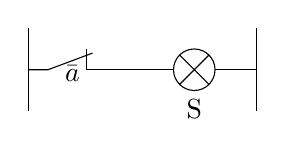
\begin{tikzpicture}[x=0.75pt,y=0.75pt,yscale=-1,xscale=1]
%uncomment if require: \path (0,300); %set diagram left start at 0, and has height of 300

%Straight Lines [id:da8815065759848859] 
\draw    (170,50) -- (170,90) ;
%Straight Lines [id:da1350968670020839] 
\draw    (210,70) -- (240,70) ;
%Flowchart: Summing Junction [id:dp35636284771857807] 
\draw   (240,70) .. controls (240,64.48) and (244.48,60) .. (250,60) .. controls (255.52,60) and (260,64.48) .. (260,70) .. controls (260,75.52) and (255.52,80) .. (250,80) .. controls (244.48,80) and (240,75.52) .. (240,70) -- cycle ; \draw   (242.93,62.93) -- (257.07,77.07) ; \draw   (257.07,62.93) -- (242.93,77.07) ;
%Straight Lines [id:da2542947637154732] 
\draw    (260,70) -- (280,70) ;
%Straight Lines [id:da5354667804813708] 
\draw    (280,50) -- (280,90) ;
%Straight Lines [id:da23878024972148482] 
\draw    (200.95,62) -- (179.52,70) -- (170,70) ;
%Straight Lines [id:da9493501830816764] 
\draw    (198.1,60) -- (198.1,70) -- (210,70) ;


% Text Node
\draw (250,83) node [anchor=north] [inner sep=0.75pt]   [align=left] {S};
% Text Node
\draw (191.25,66.75) node [anchor=north] [inner sep=0.75pt]   [align=left] {\(\bar{a}\)};


\end{tikzpicture}}}
\\
\cmidrule(lr){4-6}
& \multicolumn{2}{c}{} & & 0 & 1 & & & & \\
& \multicolumn{2}{c}{} & & 1 & 0 & & & & \\



















\multicolumn{10}{l}{Fonction ET} \\
\middashrule
 & S	& a \cdot b	&	a & b &S	&	
 \multirow[t]{5}{=}{\vspace{-\baselineskip}
 	 \begin{compactitemize}
 	 \item commutative\,;
 	 \item associative\,;
 	 \item distributive.
 	 \end{compactitemize}}
 
 
 & \multirow[t]{5}{=}{\vspace{-\baselineskip}
 	 \begin{tabdescription}
 	 \item [élément neutre :] \(a\cdot 1=a\)
 	 \item [élément absorbant :] \(a\cdot 0=0\) 	
 	 \item [idempotence :] \(a\cdot a=a\) 	
 		\item [complément :] \(a\cdot \bar{a}=0\) 	
 	 \end{tabdescription}}
 
 
 
 
 &	\multirow[c]{5}{*}{\adjustbox{valign=t}{






\tikzset{every picture/.style={line width=0.75pt}} %set default line width to 0.75pt        

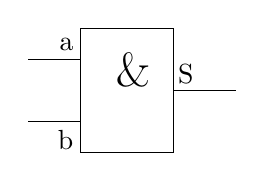
\begin{tikzpicture}[x=0.75pt,y=0.75pt,yscale=-1,xscale=1]
%uncomment if require: \path (0,300); %set diagram left start at 0, and has height of 300

%Straight Lines [id:da5742005836382655] 
\draw    (285,74.02) -- (310,74.02) ;
%Shape: Rectangle [id:dp567287790223295] 
\draw   (310,59.02) -- (355,59.02) -- (355,119.02) -- (310,119.02) -- cycle ;
%Straight Lines [id:da6580711403152724] 
\draw    (285,104.02) -- (310,104.02) ;
%Straight Lines [id:da7544895235816761] 
\draw    (355,89.02) -- (385,89.02) ;



% Text Node
\draw (308,107.02) node [anchor=north east] [inner sep=0.75pt]   [align=left] {b};
% Text Node
\draw (356,87.02) node [anchor=south west] [inner sep=0.75pt]   [align=left] {S};
% Text Node
\draw (308,71.02) node [anchor=south east] [inner sep=0.75pt]   [align=left] {a};
% Text Node
\draw (326,70.02) node [anchor=north west][inner sep=0.75pt]  [font=\LARGE] [align=left] {\&};


\end{tikzpicture}}}


&

\multirow[c]{5}{*}{\adjustbox{valign=t}{




\tikzset{every picture/.style={line width=0.75pt}} %set default line width to 0.75pt        

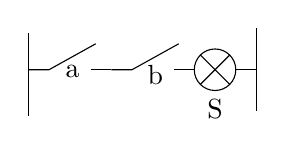
\begin{tikzpicture}[x=0.75pt,y=0.75pt,yscale=-1,xscale=1]
%uncomment if require: \path (0,300); %set diagram left start at 0, and has height of 300

%Straight Lines [id:da44167984402790095] 
\draw    (332.5,57.5) -- (310,70) -- (300,70) ;
%Straight Lines [id:da9385492498510498] 
\draw    (330,70) -- (340,70) ;

%Straight Lines [id:da5568944025291945] 
\draw    (300,52.5) -- (300,92.5) ;
%Flowchart: Summing Junction [id:dp3500177759521277] 
\draw   (380,70) .. controls (380,64.48) and (384.48,60) .. (390,60) .. controls (395.52,60) and (400,64.48) .. (400,70) .. controls (400,75.52) and (395.52,80) .. (390,80) .. controls (384.48,80) and (380,75.52) .. (380,70) -- cycle ; \draw   (382.93,62.93) -- (397.07,77.07) ; \draw   (397.07,62.93) -- (382.93,77.07) ;
%Straight Lines [id:da271209677182216] 
\draw    (400,70) -- (410,70) ;
%Straight Lines [id:da9909416639492996] 
\draw    (410,50) -- (410,90) ;
%Straight Lines [id:da7053671427847741] 
\draw    (372.5,57.5) -- (350,70) -- (340,70) ;
%Straight Lines [id:da10801947311466154] 
\draw    (370,70) -- (380,70) ;


% Text Node
\draw (390,83) node [anchor=north] [inner sep=0.75pt]   [align=left] {S};
% Text Node
\draw (321.25,66.75) node [anchor=north] [inner sep=0.75pt]   [align=left] {a};
% Text Node
\draw (361.25,66.75) node [anchor=north] [inner sep=0.75pt]   [align=left] {b};


\end{tikzpicture}}}
\\
\cmidrule(lr){4-6}
& \multicolumn{2}{c}{} & 0 & 0 & 0 & & & & \\
& \multicolumn{2}{c}{} &	0 & 1 & 0 & & & & \\
& \multicolumn{2}{c}{} &	1 & 0 & 0 & & & & \\
& \multicolumn{2}{c}{} &	1 & 1 & 1 & & & & \\











\multicolumn{10}{l}{Fonction OU} \\
\middashrule
 & S	& a + b	&	a & b &  S & \multirow[t]{5}{=}{\vspace{-\baselineskip}
 	 \begin{compactitemize}
 	 \item commutative\,;
 	 \item associative\,;
 	 \item distributive.
 	 \end{compactitemize}}

&	\multirow[t]{5}{=}{\vspace{-\baselineskip}
 	 \begin{tabdescription}
 	 \item [élément neutre :] \(a + 1=a\)
 	 \item [élément absorbant :] \(a + 1=1\) 	
 	 \item [idempotence :] \(a + a=a\) 	
 		\item [complément :] \(a + \bar{a}=1\) 	
 	 \end{tabdescription}}
&

\multirow[c]{5}*{\adjustbox{valign=t}{





\tikzset{every picture/.style={line width=0.75pt}} %set default line width to 0.75pt        

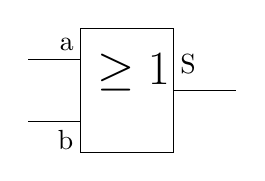
\begin{tikzpicture}[x=0.75pt,y=0.75pt,yscale=-1,xscale=1]
%uncomment if require: \path (0,300); %set diagram left start at 0, and has height of 300

%Straight Lines [id:da06752696413547643] 
\draw    (505,47) -- (530,47) ;
%Shape: Rectangle [id:dp8374388999072278] 
\draw   (530,32) -- (575,32) -- (575,92) -- (530,92) -- cycle ;
%Straight Lines [id:da9488264651646036] 
\draw    (505,77) -- (530,77) ;
%Straight Lines [id:da45735601301360473] 
\draw    (575,62) -- (605,62) ;


% Text Node
\draw (528,44) node [anchor=south east] [inner sep=0.75pt]   [align=left] {a};
% Text Node
\draw (577,55) node [anchor=south west] [inner sep=0.75pt]   [align=left] {S};
% Text Node
\draw (528,80) node [anchor=north east] [inner sep=0.75pt]   [align=left] {b};
% Text Node
\draw (537,43) node [anchor=north west][inner sep=0.75pt]  [font=\LARGE] [align=left] {\(\geq1\)};


\end{tikzpicture}}}


&

\multirow[c]{5}*{\adjustbox{valign=t}{
\tikzset{every picture/.style={line width=0.75pt}} %set default line width to 0.75pt        

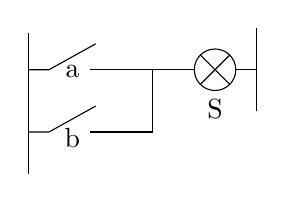
\begin{tikzpicture}[x=0.75pt,y=0.75pt,yscale=-1,xscale=1]
%uncomment if require: \path (0,300); %set diagram left start at 0, and has height of 300

%Straight Lines [id:da3256967182481336] 
\draw    (102.5,27.5) -- (80,40) -- (70,40) ;
%Straight Lines [id:da5739964470502629] 
\draw    (100,40) -- (110,40) ;

%Straight Lines [id:da5834086968565423] 
\draw    (70,22.5) -- (70,90) ;
%Flowchart: Summing Junction [id:dp19689264489217084] 
\draw   (150,40) .. controls (150,34.48) and (154.48,30) .. (160,30) .. controls (165.52,30) and (170,34.48) .. (170,40) .. controls (170,45.52) and (165.52,50) .. (160,50) .. controls (154.48,50) and (150,45.52) .. (150,40) -- cycle ; \draw   (152.93,32.93) -- (167.07,47.07) ; \draw   (167.07,32.93) -- (152.93,47.07) ;
%Straight Lines [id:da5100099011545352] 
\draw    (170,40) -- (180,40) ;
%Straight Lines [id:da5301747358856375] 
\draw    (180,20) -- (180,60) ;
%Straight Lines [id:da8660333272321838] 
\draw    (102.5,57.5) -- (80,70) -- (70,70) ;
%Straight Lines [id:da13399082746704993] 
\draw    (100,70) -- (110,70) ;

%Straight Lines [id:da41765610732090575] 
\draw    (110,40) -- (150,40) ;
%Straight Lines [id:da6952650852764948] 
\draw    (110,70) -- (130,70) -- (130,40) ;

% Text Node
\draw (160,53) node [anchor=north] [inner sep=0.75pt]   [align=left] {S};
% Text Node
\draw (91.25,36.75) node [anchor=north] [inner sep=0.75pt]   [align=left] {a};
% Text Node
\draw (91.25,66.75) node [anchor=north] [inner sep=0.75pt]   [align=left] {b};


\end{tikzpicture}}}
\\
\cmidrule(lr){4-6}
& \multicolumn{2}{c}{} & 0 & 0 & 0 & & & & \\
& \multicolumn{2}{c}{} &	0 & 1 & 1 & & & & \\
& \multicolumn{2}{c}{} &	1 & 0 & 1 & & & & \\
& \multicolumn{2}{c}{} &	1 & 1 & 1 & & & & \\











\multicolumn{10}{l}{Fonction NAND (NON-ET)} \\
\middashrule
 & S	& \overline{a \cdot b}	&	a & b &  S & 
 	 \begin{compactitemize}
 	 \item commutative.
 	 \end{compactitemize}

&	\multirow[t]{5}{=}{\vspace{-\baselineskip}
 	 \begin{compactitemize}
 	 \item \(\overline{a\cdot 1}=\bar{a}\)
 	 \item \(\overline{a\cdot 0}=1\) 	
 	 \item \(\overline{a\cdot a}=\bar{a}\) 	
 	\item \(\overline{a\cdot \bar{a}}=0\) 	
 	 \end{compactitemize}}
&

\multirow[c]{5}*{\adjustbox{valign=t}{



\tikzset{every picture/.style={line width=0.75pt}} %set default line width to 0.75pt        

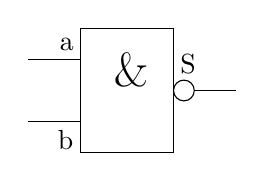
\begin{tikzpicture}[x=0.75pt,y=0.75pt,yscale=-1,xscale=1]
%uncomment if require: \path (0,300); %set diagram left start at 0, and has height of 300

%Straight Lines [id:da3075310431165378] 
\draw    (395,47) -- (420,47) ;
%Shape: Rectangle [id:dp34074320540335523] 
\draw   (420,32) -- (465,32) -- (465,92) -- (420,92) -- cycle ;
%Shape: Circle [id:dp137731335343246] 
\draw   (465,62) .. controls (465,59.24) and (467.24,57) .. (470,57) .. controls (472.76,57) and (475,59.24) .. (475,62) .. controls (475,64.76) and (472.76,67) .. (470,67) .. controls (467.24,67) and (465,64.76) .. (465,62) -- cycle ;
%Straight Lines [id:da5487960832830293] 
\draw    (395,77) -- (420,77) ;
%Straight Lines [id:da20528045761602165] 
\draw    (475,62) -- (495,62) ;


% Text Node
\draw (418,44) node [anchor=south east] [inner sep=0.75pt]   [align=left] {a};
% Text Node
\draw (467,55) node [anchor=south west] [inner sep=0.75pt]   [align=left] {S};
% Text Node
\draw (418,80) node [anchor=north east] [inner sep=0.75pt]   [align=left] {b};
% Text Node
\draw (435,43) node [anchor=north west][inner sep=0.75pt]  [font=\LARGE] [align=left] {\&};


\end{tikzpicture}}}


&

\multirow[c]{5}*{\adjustbox{valign=t}{


\tikzset{every picture/.style={line width=0.75pt}} %set default line width to 0.75pt        

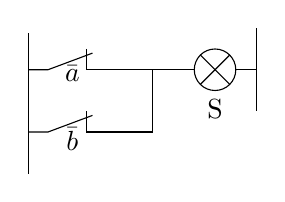
\begin{tikzpicture}[x=0.75pt,y=0.75pt,yscale=-1,xscale=1]
%uncomment if require: \path (0,300); %set diagram left start at 0, and has height of 300

%Straight Lines [id:da5834086968565423] 
\draw    (70,22.5) -- (70,90) ;
%Flowchart: Summing Junction [id:dp19689264489217084] 
\draw   (150,40) .. controls (150,34.48) and (154.48,30) .. (160,30) .. controls (165.52,30) and (170,34.48) .. (170,40) .. controls (170,45.52) and (165.52,50) .. (160,50) .. controls (154.48,50) and (150,45.52) .. (150,40) -- cycle ; \draw   (152.93,32.93) -- (167.07,47.07) ; \draw   (167.07,32.93) -- (152.93,47.07) ;
%Straight Lines [id:da5100099011545352] 
\draw    (170,40) -- (180,40) ;
%Straight Lines [id:da5301747358856375] 
\draw    (180,20) -- (180,60) ;
%Straight Lines [id:da41765610732090575] 
\draw    (110,40) -- (150,40) ;
%Straight Lines [id:da6952650852764948] 
\draw    (110,70) -- (130,70) -- (130,40) ;
%Straight Lines [id:da9259802766613583] 
\draw    (100.95,32) -- (79.52,40) -- (70,40) ;
%Straight Lines [id:da35326606444128883] 
\draw    (98.1,30) -- (98.1,40) -- (110,40) ;

%Straight Lines [id:da7829828965774251] 
\draw    (100.95,62) -- (79.52,70) -- (70,70) ;
%Straight Lines [id:da6531978729413752] 
\draw    (98.1,60) -- (98.1,70) -- (110,70) ;


% Text Node
\draw (160,53) node [anchor=north] [inner sep=0.75pt]   [align=left] {S};
% Text Node
\draw (91.25,36.75) node [anchor=north] [inner sep=0.75pt]   [align=left] {\(\bar{a}\)};
% Text Node
\draw (91.25,66.75) node [anchor=north] [inner sep=0.75pt]   [align=left] {\(\bar{b}\)};


\end{tikzpicture}}}
\\
\cmidrule(lr){4-6}
& S & \bar{a}\cdot \bar{b} & 0 & 0 & 1 & & & & \\
& \multicolumn{2}{c}{} &	0 & 1 & 1 & & & & \\
& \multicolumn{2}{c}{} &	1 & 0 & 1 & & & & \\
& \multicolumn{2}{c}{} &	1 & 1 & 0 & & & & \\










\multicolumn{10}{l}{Fonction NOR (NON-OU)} \\
\middashrule
 & S	& \overline{a / b}	&	a & b &  S & 
 	 \begin{compactitemize}
 	 \item commutative.
 	 \end{compactitemize}

&	\multirow[t]{5}{=}{\vspace{-\baselineskip}
 	 \begin{compactitemize}
 	 \item \(\overline{a + 1}=0\)
 	 \item \(\overline{a + 0}=\bar{a}\) 	
 	 \item \(\overline{a + a}=\bar{a}\) 	
 	\item \(\overline{a + \bar{a}}=0\) 	
 	 \end{compactitemize}}
&

\multirow[c]{5}*{\adjustbox{valign=t}{



\tikzset{every picture/.style={line width=0.75pt}} %set default line width to 0.75pt        

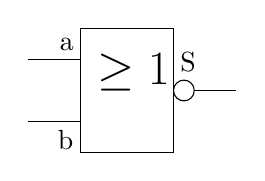
\begin{tikzpicture}[x=0.75pt,y=0.75pt,yscale=-1,xscale=1]
%uncomment if require: \path (0,300); %set diagram left start at 0, and has height of 300

%Straight Lines [id:da28054130737378413] 
\draw    (295,140) -- (320,140) ;
%Shape: Rectangle [id:dp593795280802214] 
\draw   (320,125) -- (365,125) -- (365,185) -- (320,185) -- cycle ;
%Shape: Circle [id:dp6114322437775147] 
\draw   (365,155) .. controls (365,152.24) and (367.24,150) .. (370,150) .. controls (372.76,150) and (375,152.24) .. (375,155) .. controls (375,157.76) and (372.76,160) .. (370,160) .. controls (367.24,160) and (365,157.76) .. (365,155) -- cycle ;
%Straight Lines [id:da560098762378927] 
\draw    (295,170) -- (320,170) ;
%Straight Lines [id:da6768060203685787] 
\draw    (375,155) -- (395,155) ;


% Text Node
\draw (327,136) node [anchor=north west][inner sep=0.75pt]  [font=\LARGE] [align=left] {\(\geq1\)};
% Text Node
\draw (318,173) node [anchor=north east] [inner sep=0.75pt]   [align=left] {b};
% Text Node
\draw (367,147) node [anchor=south west] [inner sep=0.75pt]   [align=left] {S};
% Text Node
\draw (318,137) node [anchor=south east] [inner sep=0.75pt]   [align=left] {a};


\end{tikzpicture}}}


&

\multirow[c]{5}*{\adjustbox{valign=t}{



\tikzset{every picture/.style={line width=0.75pt}} %set default line width to 0.75pt        

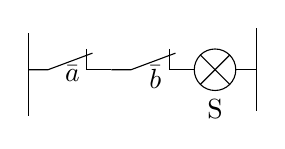
\begin{tikzpicture}[x=0.75pt,y=0.75pt,yscale=-1,xscale=1]
%uncomment if require: \path (0,300); %set diagram left start at 0, and has height of 300

%Straight Lines [id:da532813825776433] 
\draw    (170,72.5) -- (170,112.5) ;
%Flowchart: Summing Junction [id:dp6472344153140596] 
\draw   (250,90) .. controls (250,84.48) and (254.48,80) .. (260,80) .. controls (265.52,80) and (270,84.48) .. (270,90) .. controls (270,95.52) and (265.52,100) .. (260,100) .. controls (254.48,100) and (250,95.52) .. (250,90) -- cycle ; \draw   (252.93,82.93) -- (267.07,97.07) ; \draw   (267.07,82.93) -- (252.93,97.07) ;
%Straight Lines [id:da41670520625879814] 
\draw    (270,90) -- (280,90) ;
%Straight Lines [id:da8475403662444542] 
\draw    (280,70) -- (280,110) ;
%Straight Lines [id:da7699507171424776] 
\draw    (200.95,82) -- (179.52,90) -- (170,90) ;
%Straight Lines [id:da40034423236269534] 
\draw    (198.1,80) -- (198.1,90) -- (210,90) ;

%Straight Lines [id:da8026199631794467] 
\draw    (240.95,82) -- (219.52,90) -- (210,90) ;
%Straight Lines [id:da4591243198185887] 
\draw    (238.1,80) -- (238.1,90) -- (250,90) ;


% Text Node
\draw (260,103) node [anchor=north] [inner sep=0.75pt]   [align=left] {S};
% Text Node
\draw (191.25,86.75) node [anchor=north] [inner sep=0.75pt]   [align=left] {\(\bar{a}\)};
% Text Node
\draw (231.25,86.75) node [anchor=north] [inner sep=0.75pt]   [align=left] {\(\bar{b}\)};


\end{tikzpicture}}}
\\
\cmidrule(lr){4-6}
& S & \bar{a} \cdot \bar{b} & 0 & 0 & 1 & & & & \\
& \multicolumn{2}{c}{} &	0 & 1 & 0 & & & & \\
& \multicolumn{2}{c}{} &	1 & 0 & 0 & & & & \\
& \multicolumn{2}{c}{} &	1 & 1 & 0 & & & & \\








\multicolumn{10}{l}{Fonction XOR} \\
\middashrule
 & S	& a \oplus b	&	a & b &  S & 
 	 \begin{compactitemize}
 	 \item commutative\,;
 	 \item associative
 	 \end{compactitemize}

&	\multirow[t]{5}{=}{\vspace{-\baselineskip}
 	 \begin{compactitemize}
 	 \item \(a \oplus 1=\bar{a}\)
 	 \item \(a \oplus 0=a\) 	
 	 \item \(a \oplus a=0\) 	
 	\item \(a \oplus \bar{a}=0\) 	
 	 \end{compactitemize}}
&

\multirow[c]{5}*{\adjustbox{valign=t}{




\tikzset{every picture/.style={line width=0.75pt}} %set default line width to 0.75pt        

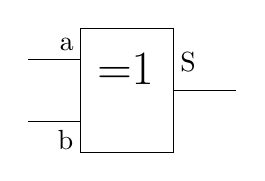
\begin{tikzpicture}[x=0.75pt,y=0.75pt,yscale=-1,xscale=1]
%uncomment if require: \path (0,300); %set diagram left start at 0, and has height of 300

%Straight Lines [id:da08283118091038022] 
\draw    (175,140) -- (200,140) ;
%Shape: Rectangle [id:dp4077631643544083] 
\draw   (200,125) -- (245,125) -- (245,185) -- (200,185) -- cycle ;
%Straight Lines [id:da8844255042506907] 
\draw    (175,170) -- (200,170) ;
%Straight Lines [id:da7167492043179563] 
\draw    (245,155) -- (275,155) ;


% Text Node
\draw (198,137) node [anchor=south east] [inner sep=0.75pt]   [align=left] {a};
% Text Node
\draw (247,147) node [anchor=south west] [inner sep=0.75pt]   [align=left] {S};
% Text Node
\draw (198,173) node [anchor=north east] [inner sep=0.75pt]   [align=left] {b};
% Text Node
\draw (207,136) node [anchor=north west][inner sep=0.75pt]  [font=\LARGE] [align=left] {=1};


\end{tikzpicture}


}}


&

\multirow[c]{5}*{\adjustbox{valign=t}{

\tikzset{every picture/.style={line width=0.75pt}} %set default line width to 0.75pt        

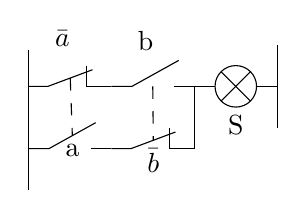
\begin{tikzpicture}[x=0.75pt,y=0.75pt,yscale=-1,xscale=1]
%uncomment if require: \path (0,300); %set diagram left start at 0, and has height of 300

%Straight Lines [id:da6778149503103992] 
\draw    (492.5,57.5) -- (470,70) -- (460,70) ;
%Straight Lines [id:da4005632802005663] 
\draw    (490,70) -- (500,70) ;

%Straight Lines [id:da7736081033781883] 
\draw    (420,52.5) -- (420,120) ;
%Flowchart: Summing Junction [id:dp25956302339936166] 
\draw   (510,70) .. controls (510,64.48) and (514.48,60) .. (520,60) .. controls (525.52,60) and (530,64.48) .. (530,70) .. controls (530,75.52) and (525.52,80) .. (520,80) .. controls (514.48,80) and (510,75.52) .. (510,70) -- cycle ; \draw   (512.93,62.93) -- (527.07,77.07) ; \draw   (527.07,62.93) -- (512.93,77.07) ;
%Straight Lines [id:da6093803763449405] 
\draw    (530,70) -- (540,70) ;
%Straight Lines [id:da31479906060868335] 
\draw    (540,50) -- (540,90) ;
%Straight Lines [id:da8748426220885159] 
\draw    (490.95,92) -- (469.52,100) -- (460,100) ;
%Straight Lines [id:da5799707886976846] 
\draw    (488.1,90) -- (488.1,100) -- (500,100) ;

%Straight Lines [id:da4718489453418031] 
\draw    (452.5,87.5) -- (430,100) -- (420,100) ;
%Straight Lines [id:da06798618040851889] 
\draw    (450,100) -- (460,100) ;

%Straight Lines [id:da792550075176628] 
\draw    (450.95,62) -- (429.52,70) -- (420,70) ;
%Straight Lines [id:da9873390703902969] 
\draw    (448.1,60) -- (448.1,70) -- (460,70) ;

%Straight Lines [id:da3601015213239418] 
\draw    (500,100) -- (500,70) -- (510,70) ;
%Straight Lines [id:da21859666404808997] 
\draw  [dash pattern={on 4.5pt off 4.5pt}]  (440.24,66) -- (441.25,93.75) ;
%Straight Lines [id:da1706765920441512] 
\draw  [dash pattern={on 4.5pt off 4.5pt}]  (480,70) -- (480.24,96) ;

% Text Node
\draw (520,83) node [anchor=north] [inner sep=0.75pt]   [align=left] {S};
% Text Node
\draw (436.5,42) node [anchor=north] [inner sep=0.75pt]   [align=left] {\(\bar{a}\)};
% Text Node
\draw (480.24,99) node [anchor=north] [inner sep=0.75pt]   [align=left] {\(\bar{b}\)};
% Text Node
\draw (441.25,96.75) node [anchor=north] [inner sep=0.75pt]   [align=left] {a};
% Text Node
\draw (476.5,42) node [anchor=north] [inner sep=0.75pt]   [align=left] {b};


\end{tikzpicture}}}
\\
\cmidrule(lr){4-6}
& S & \bar{a} \cdot b + a \cdot \bar{b} & 0 & 0 & 1 & & & & \\
& \multicolumn{2}{c}{} &	0 & 1 & 1 & & & & \\
& \multicolumn{2}{c}{} &	1 & 0 & 1 & & & & \\
& \multicolumn{2}{c}{} &	1 & 1 & 0 & & & & \\









\multicolumn{10}{l}{Fonction XNOR} \\
\middashrule
 & S	& a \odot b	&	a & b &  S & 
 	 \begin{compactitemize}
 	 \item commutative.
 	  	 \end{compactitemize}

&	\multirow[t]{5}{=}{\vspace{-\baselineskip}
 	 \begin{compactitemize}
 	 \item \(a \odot 1=a\)
 	 \item \(a \odot 0=\bar{a}\) 	
 	 \item \(a \odot a=1\) 	
 	\item \(a \odot \bar{a}=0\) 	
 	 \end{compactitemize}}
&

\multirow[c]{5}*{\adjustbox{valign=t}{




\tikzset{every picture/.style={line width=0.75pt}} %set default line width to 0.75pt        

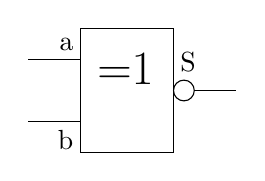
\begin{tikzpicture}[x=0.75pt,y=0.75pt,yscale=-1,xscale=1]
%uncomment if require: \path (0,300); %set diagram left start at 0, and has height of 300

%Straight Lines [id:da4641846839343067] 
\draw    (55,135) -- (80,135) ;
%Shape: Rectangle [id:dp040925003468690546] 
\draw   (80,120) -- (125,120) -- (125,180) -- (80,180) -- cycle ;
%Shape: Circle [id:dp9916692428437459] 
\draw   (125,150) .. controls (125,147.24) and (127.24,145) .. (130,145) .. controls (132.76,145) and (135,147.24) .. (135,150) .. controls (135,152.76) and (132.76,155) .. (130,155) .. controls (127.24,155) and (125,152.76) .. (125,150) -- cycle ;
%Straight Lines [id:da14336423787612584] 
\draw    (55,165) -- (80,165) ;
%Straight Lines [id:da9878364150723613] 
\draw    (135,150) -- (155,150) ;


% Text Node
\draw (78,132) node [anchor=south east] [inner sep=0.75pt]   [align=left] {a};
% Text Node
\draw (127,142) node [anchor=south west] [inner sep=0.75pt]   [align=left] {S};
% Text Node
\draw (78,168) node [anchor=north east] [inner sep=0.75pt]   [align=left] {b};
% Text Node
\draw (87,131) node [anchor=north west][inner sep=0.75pt]  [font=\LARGE] [align=left] {=1};


\end{tikzpicture}


}}


&

\multirow[c]{5}*{\adjustbox{valign=t}{


\tikzset{every picture/.style={line width=0.75pt}} %set default line width to 0.75pt        

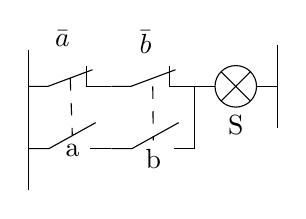
\begin{tikzpicture}[x=0.75pt,y=0.75pt,yscale=-1,xscale=1]
%uncomment if require: \path (0,300); %set diagram left start at 0, and has height of 300

%Straight Lines [id:da5241511737217781] 
\draw    (50,132.5) -- (50,200) ;
%Flowchart: Summing Junction [id:dp22324272414776847] 
\draw   (140,150) .. controls (140,144.48) and (144.48,140) .. (150,140) .. controls (155.52,140) and (160,144.48) .. (160,150) .. controls (160,155.52) and (155.52,160) .. (150,160) .. controls (144.48,160) and (140,155.52) .. (140,150) -- cycle ; \draw   (142.93,142.93) -- (157.07,157.07) ; \draw   (157.07,142.93) -- (142.93,157.07) ;
%Straight Lines [id:da7465504040251878] 
\draw    (160,150) -- (170,150) ;
%Straight Lines [id:da7165580908721336] 
\draw    (170,130) -- (170,170) ;
%Straight Lines [id:da5114706326946257] 
\draw    (120.95,142) -- (99.52,150) -- (90,150) ;
%Straight Lines [id:da3430914959653203] 
\draw    (118.1,140) -- (118.1,150) -- (130,150) ;

%Straight Lines [id:da8924516778891433] 
\draw    (82.5,167.5) -- (60,180) -- (50,180) ;
%Straight Lines [id:da7562329481778607] 
\draw    (80,180) -- (90,180) ;

%Straight Lines [id:da6206766489306966] 
\draw    (80.95,142) -- (59.52,150) -- (50,150) ;
%Straight Lines [id:da6699120239341876] 
\draw    (78.1,140) -- (78.1,150) -- (90,150) ;

%Straight Lines [id:da44203989238574215] 
\draw    (130,180) -- (130,150) -- (140,150) ;
%Straight Lines [id:da40048100450943946] 
\draw  [dash pattern={on 4.5pt off 4.5pt}]  (70.24,146) -- (71.25,173.75) ;
%Straight Lines [id:da580856620365253] 
\draw  [dash pattern={on 4.5pt off 4.5pt}]  (110,150) -- (110.24,176) ;
%Straight Lines [id:da42117934147167313] 
\draw    (122.5,167.5) -- (100,180) -- (90,180) ;
%Straight Lines [id:da6073516596183609] 
\draw    (120,180) -- (130,180) ;


% Text Node
\draw (150,163) node [anchor=north] [inner sep=0.75pt]   [align=left] {S};
% Text Node
\draw (66.5,122) node [anchor=north] [inner sep=0.75pt]   [align=left] {\(\bar{a}\)};
% Text Node
\draw (110.24,179) node [anchor=north] [inner sep=0.75pt]   [align=left] {b};
% Text Node
\draw (71.25,176.75) node [anchor=north] [inner sep=0.75pt]   [align=left] {a};
% Text Node
\draw (106.5,122) node [anchor=north] [inner sep=0.75pt]   [align=left] {\(\bar{b}\)};


\end{tikzpicture}
}}
\\
\cmidrule(lr){4-6}
& S & a \cdot b + \bar{a} \cdot \bar{b} & 0 & 0 & 1 & & & & \\
& S	& \overline{a \oplus b}  &	0 & 1 & 0  & & & & \\
& \multicolumn{2}{c}{} &	1 & 0 & 0 & & & & \\
& \multicolumn{2}{c}{} &	1 & 1 & 1 & & & & \\




\end{longtableau}
 \end{landscape}


\end{document}

